%!TEX root = ../../main.tex

\chapter{Project Planning}
In order to control the flow of the project, the V-Model approach was taken. The
project is therefore divided into Requirements, System Design, Architecture Design,
Module Design and Implementation. After Implementation the corresponding
verification phases are ready to be executed, starting from the lowest level (Unit
Verification) to Integration Verification, System Verification and last but not least
Acceptance Verification.


\begin{figure}[h]
\centering
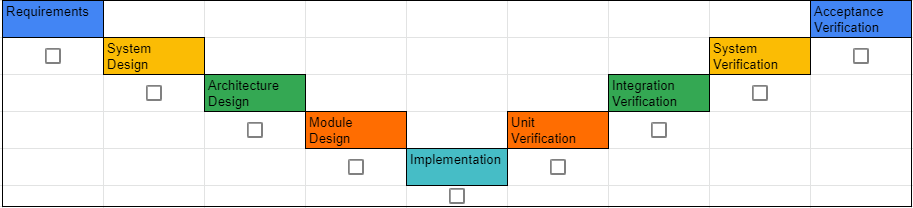
\includegraphics[scale=0.65]{vmod.png}
\caption{V-Model}
\end{figure}

At the beginning of every project phase, workloads were defined e.g. the definition of
the Control Unit Entity. The target of Requirements Engineering was to define
everything that is expected from the core and gather information about RISC-V. The
data path as well as the entities of the Control Unit, Arithmetic Unit, Register Files,
Exception Control, \acs{PMP} \& \acs{PMA} Checker and AXI4-Lite Interfaces as well as a short
summary of their function were defined during System Design. The next step,
Architecture Design, aimed to further specify the entities mentioned above and
sub-divide them into several entities. Module Design will be executed to define every
single architecture, after that implementation and testing may start.
